

\begin{table*}[t]
\caption{Images, Lesions, Median Age per Lesion, and Median Saturation and Lesion-to-Skin $\Delta E$ per Image, by Class and Source (Ros: rosendahl, Mod: vidir\_modern, Mol: vidir\_molemax, Dias: vienna\_dias)}
\label{tab:classes}
\centering
\footnotesize
\begin{tabular}{lrrr|ccccc|ccccc}
\hline
& & & & \multicolumn{5}{c|}{Saturation} & \multicolumn{5}{c}{$\Delta E$} \\
Class & Images & Lesions & Age & All & Ros & Mod & Mol & Dias & All & Ros & Mod & Mol & Dias \\
\hline
Melanocytic nevus (nv) & 6705 & 5403 & 45 & .360 & .210 & .198 & .423 & .313 & 26.6 & 27.0 & 33.0 & 24.6 & 31.8 \\
Melanoma (mel) & 1113 & 614 & 65 & .250 & .262 & .235 & .387 & .337 & 28.1 & 23.1 & 29.7 & 32.3 & 31.9 \\
Benign keratosis (bkl) & 1099 & 727 & 65 & .226 & .209 & .219 & .372 & .281 & 16.2 & 13.2 & 19.0 & 18.3 & 23.9 \\
Basal cell carcinoma (bcc) & 514 & 327 & 70 & .215 & .223 & .206 & -- & -- & 11.0 & 9.8 & 12.9 & -- & -- \\
Actinic keratosis / IEC (akiec) & 327 & 228 & 67.5 & .264 & .265 & .250 & -- & -- & 10.9 & 10.9 & 10.5 & -- & -- \\
Vascular lesion (vasc) & 142 & 98 & 55 & .249 & -- & .212 & .330 & -- & 32.3 & -- & 30.4 & 33.0 & -- \\
Dermatofibroma (df) & 115 & 73 & 55 & .245 & .218 & .218 & .351 & -- & 15.0 & 11.0 & 18.5 & 14.0 & -- \\
\hline
All & 10015 & 7470 & 50 & .291 & .227 & .211 & .420 & .320 & 24.8 & 17.3 & 28.8 & 24.5 & 31.5 \\
\hline
\end{tabular}
\end{table*}

We use HAM10000~\cite{b2}, obtained from the Harvard Dataverse. It was collected to train and benchmark automated diagnosis of pigmented skin lesions and contains 10,015 images of 7,470 lesions from four sources in Austria and Australia.
Inputs are $600\times450$ RGB dermoscopic images (Fig.~\ref{fig:samples}) with binary lesion masks, age, sex, and body site.
Labels are seven diagnoses (Table~\ref{tab:classes}), confirmed by histopathology for 53.3\% of images and otherwise by follow-up, expert consensus, or confocal microscopy.
Classes range from 66.9\% of images for nv to 1.1\% for df, a 58:1 imbalance (Fig.~\ref{fig:classes}).

The data will be divided into training and validation folds grouped by lesion, because 44.9\% of images show lesions photographed more than once.

The RGB channel means [0.764, 0.546, 0.571] differ substantially from those of ImageNet, so ImageNet statistics will be used only for pretrained models.
Image properties differ strongly between sources (Table~\ref{tab:props}).

Source is correlated with the diagnosis: \texttt{vidir\_molemax} is 94.1\% nv and 0.6\% mel, and differs visibly in appearance from the other sources (Fig.~\ref{fig:classes}).
Class-level trends can reverse within a source (Table~\ref{tab:classes}): saturation is higher for nv than for mel overall, but lower in three of four sources, so a model may learn the source rather than the lesion itself.

Heuristically detected dark corners (vignettes) affect 26.2\% of mel but only 7.8\% of nv images, and 32.2\% of \texttt{vidir\_modern} images; hair affects 12.6\% of images.
The most extreme images in sharpness and exposure were inspected visually.

We expect vasc to be easily detectable (distinctive red hue, $\Delta E \approx 32.3$), while low-contrast akiec and bcc ($\Delta E\approx11$), mel versus nv, and rare df should be harder.
Training will use crops, flips, rotations, mild color jitter guided by source differences, and a class-independent vignette in order to avoid data poisoning by existing ones.

\begin{table}[t]
\caption{Per-Image Properties}
\label{tab:props}
\centering
\footnotesize
\setlength{\tabcolsep}{2.5pt}
\begin{tabular}{lccccc|cccc}
\hline
Property & Mean & Med & Min & Max & Std & Ros & Mod & Mol & Dias \\
\hline
Brightness & .765 & .774 & .323 & .997 & .097 & .751 & .693 & .839 & .753 \\
Contrast & .109 & .101 & .019 & .335 & .045 & .088 & .115 & .096 & .144 \\
Saturation & .306 & .291 & .035 & .710 & .118 & .227 & .211 & .420 & .320 \\
Sharpness & 1.89 & 1.83 & 0.94 & 3.68 & 0.34 & 1.93 & 1.82 & 1.76 & 2.10 \\
Near-black & 3.4 & -- & -- & -- & -- & 1.8 & 8.6 & 0.0 & 3.2 \\
\hline
\end{tabular}
\end{table}

\begin{figure}[t]
\centering
% 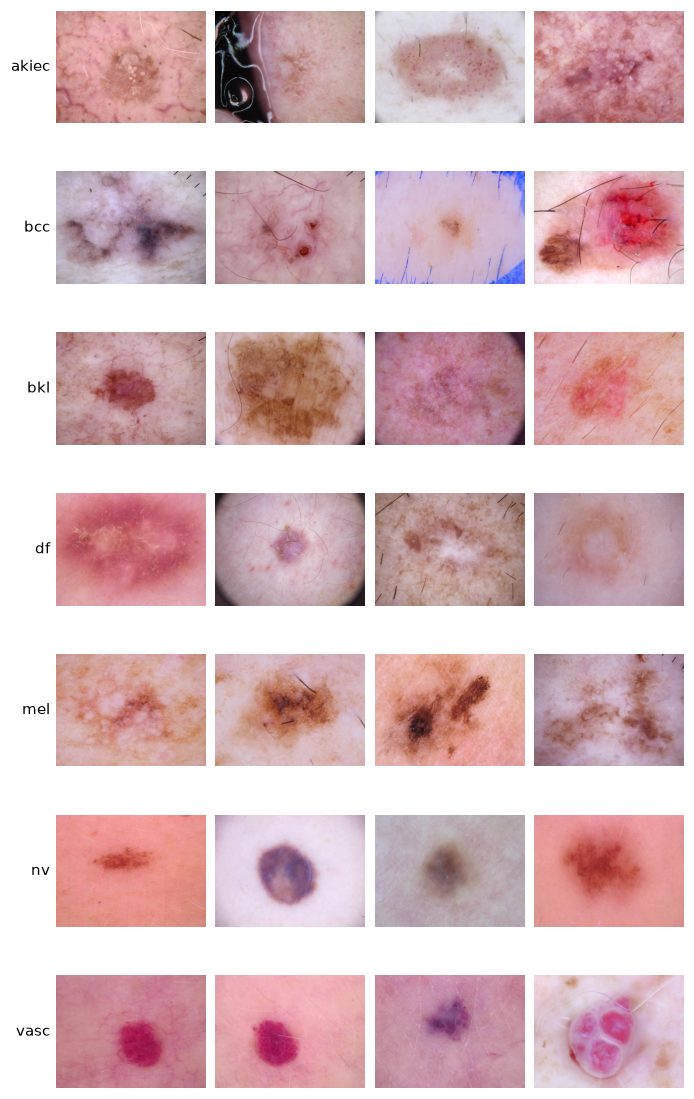
\includegraphics[width=0.6\columnwidth]{figures/samples}
\caption{Random sample images per class, one image per lesion.}
\label{fig:samples}
\end{figure}

\begin{figure}[t]
\centering
% 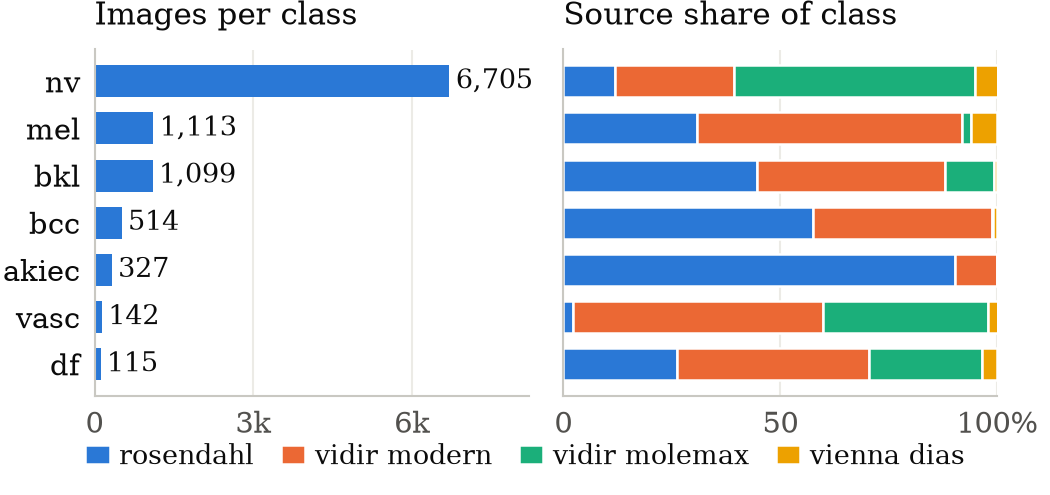
\includegraphics[width=\columnwidth]{figures/class_distribution}
\caption{Label distribution and the share of each class contributed by each source.}
\label{fig:classes}
\end{figure}
